\section{Background}
\label{sec:exposure_background}

Chapter One focused on processing, checking and exploring the spatial data that was created from the LTDS, leading to the LTDS-X. The daily journeys of around 45,000 people were recreated on a fine spatial and temporal scale from survey data. This data-set was created to allow investigation of exposure in urban environments, and also miss-classification, as described in Section \ref{sec:dynamicexposurehealth}, namely the differences between assigning someone a static exposure value based on their home location, postcode, nearest monitoring site or otherwise, compared with a model which considers all the micro-environments and varying concentrations during the subjects daily movements.

The thrust of this chapter will therefore be to link the LTDS-X dataset to the CMAQ-Urban dataset (described in \ref{sec:cmaq_urban}), and then to undertake micro-environmental modelling for when the subjects are indoors and for when they are in transport. The completed model of exposure is henceforth referred to as the London Hybrid Exposure Model or LHEM. The LHEM will then be used to explore exposure variations within the subjects, to attempt to identify and understand any patterns, and to consider exposure missclassification that may be occurring using standard exposure methods. Potential policy uses of the LHEM, and ways in which it might be useful to the general public, are then discussed.

%%%%%%%%%%%%%%%%%%%%%%%%%%%%%%%%%%%%%%%%%%%%%%%%%%%%%%%%%%%%%%%%%%%%%%%%%%%%%
\section{Methods}
\label{sec:exposure_methods}
%%%%%%%%%%%%%%%%%%%%%%%%%%%%%%%%%%%%%%%%%%%%%%%%%%%%%%%%%%%%%%%%%%%%%%%%%%%%%

In order to calculate the 'static' exposure estimates which will be compared to the LHEM estimates, a number of input data-sets and methods/processes needed to be completed. They are now listed and explained below, with the methods and input data-sets grouped by the final dataset under construction.

%%%%%%%%%%%%%%%%%%%%%%
    \subsection{Running the London Hybrid Exposure Model}
    \label{sec:running_the_lhem}
%%%%%%%%%%%%%%%%%%%%%%

        \subsubsection{Linking LTDS-X to outdoor concentrations}
        \label{sec:linking_ltdsx_to_cmaq}

During Methods section \ref{sec:cmaq_urban} the CMAQ-Urban air quality model was introduced. It was explained how this model outputs daily (weekday/Saturday/Sunday), hourly concentrations for a 20 metre by 20 metre grid covering the UK. The concentration of a range of pollutants at the location of each individuals minute-by-minute location over 24 hours was therefore now extracted from this model output i.e. the LTDS-X was linked to a CMAQ-Urban layer. Due to the memory and processing power needed to run the CMAQ-Urban model, and the language that it is written in (Fortran with SQL inputs), linking CMAQ-Urban directly to the PostgreSQL database that the LTDS-X data is held in was not possible. A CSV file of the LTDS-X in lat/long format along with a date-time-stamp was thus exported from the database. To avoid duplication at this stage, a SQL query was written to only export unique points. To explain, if someone stayed in the same location between 07:00 and 07:45 on a Saturday, only one point was exported as the temporal resolution of the CMAQ-Urban model is monthly, daily, hourly and thus the concentration at that point would not change during that time-frame. If however the same person was in constant movement between 07:00 and 07:45, then 45 points were outputted (as concentrations would be different in different locations for each minute). By taking the temporal resolution of the CMAQ-Urban model into account when doing the export query, the number of points that needed concentrations extracting from the CMAQ-Urban model was reduced from around 64 million (45,079 people multiplied by 24 hours multiplied by 60 minutes) to just over 4 million. Dr Kitwiroon of the Environmental Research Group at King's College London processed this dataset with the CMAQ-Urban model, and returned a CSV file with additional columns for a range of pollutants (including crucially NO$_{2}$ and PM$_{2.5}$). This data was then re-imported back to the PostgreSQL database and linked to the LTDS-X data.

        \subsubsection{Modelling for in-building exposure}
        \label{sec:modelling_in_building}

While LTDS-X subjects are indoors, the air quality that they are exposed to is different to outdoor air. A method to estimate exposure to outdoor air when indoors was therefore required, particularly given that subjects spend so much of their time indoors (See Figure \ref{fig:age_barplots_time_transport} in Section \ref{sec:reconstruction_results}). We decided to use an indoor/outdoor (I/O) model to estimate concentrations inside buildings, by taking ratios and applying them to the outdoor CMAQ-Urban concentrations. The model that was chosen for this was developed by Dr J. Taylor of UCL, in which he assumes 15 building types derived from the English Housing Survey, and then creates building physic models using the location of the dwelling, window opening and closing behaviour, occupant behaviour, deposition rates and penetration factors. This model was chosen as it was specifically developed for London (and therefore the building archetypes are representative), was recent (2014), and due to our close relationship with Dr Taylor meaning that we were able to ask for minor customisations to the model to be completed, and for a bestoke number of model runs to be udertaken to examine sensitivity of the model (not covered here). The methods are more fully described in \cite{Taylor2014}, and the data was  provided by personal communication with Dr Taylor (with minor customisations as mentioned  to provide hourly results and the addition of NO$_{2}$ instead of just PM). A map of the PM$_{2.5}$ ratios with the London Underground overlaid to help with the readers orientation is shown below in Figure \ref{fig:ratios_underground}.

\begin{figure}[H]
\centering
\includegraphics[scale=0.5]{ratios_underground}
\caption{Map of average indoor/outdoor (I/O) ratios used in the LHEM. Superimposed on the map is the London Underground network to aid orientation}
\label{fig:ratios_underground}
\end{figure}

            \paragraph{Importing I/O ratios}
            \label{sec:importing_io_ratios}
	
The data-set was provided as a CSV file which gave hourly I/O averages for each district level postcode in London. The data was re-organised slightly, before being imported to the PostgreSQL database.

            \paragraph{Linking postcodes boundaries to Indoor/outdoor ratios}
            \label{sec:linking_postcodes_to_ratios}

In order to link the provided I/O ratios to the locations in the LTDS-X, the areas that each postcode covers was required (the I/O file provided by Taylor contained a ratio, and a postcode i.e. SE173DA, 0.6 -- but did not contain geographical data defining the area that this postcode covers). The geographical postcode data-set that was used is described in Section \ref{sec:import_postcode_boundaries}, and linked to the ratios dataset using the postcode field common in both files.

            \paragraph{Take each point and link to the correct I/O on time/place}
            \label{sec:linking_points_to_postcode_ratios}

To then link the LTDS-X data to the postcode I/O ratios, a spatial SQL query to join the two tables was written. The join was performed using the location of the LTDS-X point, as well as the time of day (as the I/O dataset had this level of temporal resolution). This process is summarised in the bullet-points below:

\begin{enumerate}
\item Take the LTDS-X location (Easting and Northing) and locate the postcode boundary that contains the point
\item Now take the hour of the day that the LTDS-X is for (0-24)
\item Extract the I/O ratio
\end{enumerate}

            \paragraph{Multiply I/O ratio by CMAQ-Urban concentration}
            \label{sec:multiple_io_by_cmaq}

The appropriate I/O ratio was then multiplied by the CMAQ unique point value for that location, day and hour, the result being the indoor exposure at that minute. This process was repeated for all the LTDS-X data-points that are noted as being indoors in the dataset (approximately 62 million points)

        \subsubsection{Modelling for in-vehicle exposure}
        \label{sec:in_vehicle_modelling}

Locations in the LTDS-X that were recorded as travelling inside vehicles (buses, cars, trains etc.) needed further micro-environmental modelling to take into account that the air quality is different from the outside air. This concept was introduced in Section \ref{subsubsec:invehicle} and then exposure studies that considered this area of modelling and exposure were examined in Section \ref{sec:transport}. To calculate in-vehicle exposure in this model, the pollutant concentration (C$_{in}$) was derived by solving the following mass balance equation below (Equation \ref{eq:mass_balance}).

\begin{equation}
\frac{dC_{in}}{dt} = \lambda _{win} (C_{out} - C_{in}) - n\lambda _{HVAC} C_{in} - V_{g} (A\textsuperscript{*}/V) C_{in} + Q/V
\label{eq:mass_balance}
\end{equation}

\begin{itemize}
\item C$_{out}$ is the outdoor CMAQ-Urban concentration linked in Section \ref{sec:linking_ltdsx_to_cmaq}
\item $\lambda _{win}$ is the air exchange rate from the windows
\item $\lambda _{HV AC}$ is the air exchange rate from the  mechanical ventilation system
\item \textit{n} is the filter removal efficiency taking values between 0 and 1
\item V$_{g}$ is the deposition velocity in m/h$^{-1}$
\item A\textsuperscript{*} is the internal surface area available for deposition
\item V the volume of the vehicle
\item Q is the in-vehicle particle emission rate in ug/h$^{-1}$ (defined as the product of the re-suspension rate and the number of active passengers)
\end{itemize}

This was solved analytically and the general solution is shown below in Equation \ref{eq:solved_mass_balance}.

\begin{equation}
C_{in} = (C_{in_{0}} - \frac{b_{0}}{a_{0}}) \cdot exp(-a \cdot t) + \frac{b}{a}
\label{eq:solved_mass_balance}
\end{equation}

The parameters for this model change as the subjects move, and for different vehicle types. For an example of how this module of the LHEM operates, please find a standalone piece of R code in Appendix \autoref{code:in_vehicle_example}.
            
            \paragraph{The London Underground}
            \label{sec:the_london_underground}

For subjects locations in the LTDS-X that are described as being on the London Underground, fixed concentrations were used due to a lack of the data required to create a model of adequate spatial and temporal resolution. These fixed concentrations were derived from measurements conducted at underground platforms and on trains, in a separate as yet unpublished study within the Environmental Research Group at King's College London (Dr. Barratt, personal communication). For PM$_{2.5}$ the values of 94 $\mu \text{g m}^{-3}$ (winter) and 68 $\mu \text{g m}^{-3}$ (summer) were used, and for NO$_{x}$ the value of 51 $\mu \text{g m}^{-3}$ was used. n.b Chapter \ref{chap:monitoring_on_underground} aims to refine the estimation of exposure while on the London Underground. NEED TO ADD PARIS REFERENCE HERE ABOUT NO2

        \subsubsection{Summary of LTDS-X to LHEM}
        \label{sec:summary_of_ltdsx_to_lhem}

The LTDS-X data is processed, as described above, using the appropriate method for each micro-environment. Once complete a dataset of 1,440 records (24 hours x 60 minutes) including time, location and exposure is output for each individual and then the 1-minute resolution data are averaged into hour of the day or full 24 hour period to obtain the typical exposure for each individual. These are then grouped or disaggregated as appropriate depending on the analysis required.

%%%%%%%%%%%%%%%%%%%%%%
    \subsection{Creation of a postcode comparison dataset}
    \label{sec:creating_postcode_dataset}
%%%%%%%%%%%%%%%%%%%%%%

        \subsubsection{Importing postcode boundaries}
        \label{sec:import_postcode_boundaries}

To be able to calculate annual average pollutant concentrations for each London postcode, a dataset of postcodes was required, and specifically one which contains the geographical information describing the boundary of the postcode polygon. In the UK the Royal Mail is the organisation with authority for maintaining a list of all postcodes, specifically the dataset is called the Postcode Address File or PAF. However this dataset does not contain the geographical information to link the postcodes to any other spatial data. Therefore the Ordnance Survey dataset, Code-Point Open (\cite{OrdnanceSurvey2015a}), was considered. This is a dataset maintained by the Ordnance Survey, derived from the Postcode Address File, which adds the Easting and Northing of the postcode centroid to each of the Royal Mail postcodes. Although geographical coordinates now allow plotting of this dataset as points, to calculate postcode polygon averages a boundary is required, and therefore this dataset was also not suitable. Fortunately the organisation Edina, part of the "EDINA and Data Library" division of the Information Services Department at the University of Edinburgh, and funded by the UK Higher Education Authorities Joint Information and Systems Committee, has derived postcode polygon boundaries from this dataset and makes this dataset freely available to other UK Higher Education Institutions as a file called 'Code-Point with Polygons' (\cite{OrdnanceSurvey2015}). This dataset was therefore downloaded as an ESRI shapefiles and then the shp2pgsql tool used to load the shapefiles into a PostgreSQL/PostGIS database. The area of Waterloo is shown in Figure \ref{fig:postcode_polygons_example} to illustrate the detail of the final postcodes dataset.

\begin{figure}[H]
\centering
\includegraphics[scale=0.4]{postcode_polygons_example}
\caption{Postcode polygons from Edina Digimap}
\label{fig:postcode_polygons_example}
\end{figure}

        \subsubsection{Importing CMAQ-urban annual average points}
        \label{importing_cmaq_annual_averages}

To calculate the mean annual pollutant concentration within each postcode polygon, a CMAQ-Urban output file containing annual average 2011 concentrations covering a 20m x 20m grid of London was generated by Dr Kitwiroon of the Environmental Research Group at King's College London. This was imported into the PostgreSQL/PostGIS database using the raster2pgsql tool. To demonstrate this data, \ref{fig:example_cmaq_annual} and \ref{fig:example_cmaq_annual_with_postcodes} were produced by loading the data into QGIS and a colour gradient applied (and are shown below).

\begin{figure}[H]
\centering
\includegraphics[scale=0.5]{example_cmaq_annual}
\caption{CMAQ-Urban annual mean concentration raster (2011)}
\label{fig:example_cmaq_annual}
\end{figure}

\begin{figure}[H]
\centering
\includegraphics[scale=0.4]{example_cmaq_annual_with_postcodes}
\caption{CMAQ-Urban annual mean concentration raster (2011) with postcode layer}
\label{fig:example_cmaq_annual_with_postcodes}
\end{figure}

        \subsubsection{Calculating the mean concentration for each postcode}
        \label{calculating_mean_postcode_data}

To calculate the mean concentration for each postcode, the mean of the concentration of all the 20m x 20m cells that intersected the postcode were taken. Each of the LTDS subjects home address Easting and Northing was then taken, spatially joined with the postcode dataset to establish which postcode they lived in, and then the relevant annual mean concentration taken from the previously mentioned join/method.

%%%%%%%%%%%%%%%%%%%%%%
    \subsection{Creation of address-point comparison dataset}
    \label{sec:creating_address_point_dataset}
%%%%%%%%%%%%%%%%%%%%%%

To calculate the address-point comparison dataset, the home address location (Easting/Northing) of each LTDS participant was first taken, as well as the day of the week that the participant was surveyed (translated into weekday/Saturday/Sunday as this was the temporal resolution of CMAQ-Urban). This data was then extracted as a CSV for similar reasons to the section \ref{sec:linking_ltdsx_to_cmaq} and processed by Dr Kitwiroon who returned a CSV with additional columns for a range of pollutants at each location. The 24 hour average for each of the LTDS subjects addresses was then calculated for each pollutant.

%%%%%%%%%%%%%%%%%%%%%%
    \subsection{Creating of monitoring sites comparison dataset}
    \label{sec:creating_monitoring_site_dataset}
%%%%%%%%%%%%%%%%%%%%%%

        \subsubsection{Monitoring site data}
        \label{sec:monitoring_site_data}

As discussed in Section \ref{subsec:monitoringstation}, monitoring stations have often been used as a measure of exposure for a population, particularly in time-series studies e.g. \cite{Atkinson2010}, but also in some cohort studies e.g. \cite{Dockery1993}. Comparisons between the annual average of a London 'roadside' monitoring station and a London 'background' monitoring station were therefore chosen to compare with the LHEM results. The data for these sites was downloaded using OpenAir from the London Air Quality Network (\cite{LondonAir}) for the sites of Marylebone Road (roadside) and North Kensington (background) respectively (shown in Figure \ref{fig:background_roadside_monitors}).

\begin{figure}[H]
\centering
\includegraphics[scale=0.8]{background_roadside_monitors}
\caption{The monitoring stations and surrounding areas (North Kensington left, Marylebone Road right}
\label{fig:background_roadside_monitors}
\end{figure}

Specifically, the hourly means for 2011, for each site, for PM$_{2.5}$ and NO$_{2}$ were downloaded. Providing that there was at least a 75\% capture rate for the year for each pollutant (which there was) then the mean of the hours was taken as per DEFRA guidance (\cite{DEFRA2009}). The results are shown in Table \ref{tab:mean_monitoring_site_concentrations}:

\begin{table}[H]
\centering
    \begin{tabular}{ | l | l | l |}
    \hline 
     \bfseries{Site} & \bfseries{PM$_{2.5}$ ($\mu \text{g m}^{-3}$)} & \bfseries{NO$_{2}$ ($\mu \text{g m}^{-3}$}  \\ \hline
     North Kensington & 16.33 & 35.96\\ \hline
     Marylebone Road & 24.45 & 97.05\\ \hline
    \end{tabular}
\caption{Mean pollutant concentrations from London monitoring sites for 2011}
\label{tab:mean_monitoring_site_concentrations}
\end{table}

%Although the LTDS data being analysed covers questionnaires of households during the period 2005-2010, sufficient NO$_{x}$ and PM$_{2.5}$ data for a whole year, and for both the background and roadside monitoring sites, was only available for the year 2011. Therefore, as described above, this dataset was chosen for comparison (Should I calculate some other annual means for these sites to justify that using 2011 isn't much different to using 2008 or say 2010? If indeed that is the case?)

        \subsubsection{Summary}
        \label{subsubsec:methods_summary}

Now that the LHEM has been created, it allows detailed interrogation and investigation of the exposure of \textasciitilde45,000 Londoners (and the demographic and geographic information linked to them). Calculations can be made to answer many questions. To give an indication of it's capabilities, some examples are listed below:

\begin{itemize}
\item What is the average NO$_{2}$ exposure of those under 18, compared to those over 18
\item What is the average PM$_{2.5}$ exposure of people of Indian ethnic origin living in Southwark
\item What is the difference between exposure taken from monitoring sites, compared to exposure using the LHEM
\item What percentage of Londoners daily PM$_{2.5}$ exposure comes from their morning commute
\item How much less (or more?) NO$_{2}$ is someone exposed to by working at home instead of in the office
\item Which Borough of London residents have the lowest exposure
\item Is household income and air quality exposure related
\item Do children get most of their daily exposure from within 1km of their house
\item What is the difference between exposure using address-point methods, compared to exposure using the LHEM
\item During which hour of the day, do people aged between 30-40 years old get most of their daily exposure
\end{itemize}

%%%%%%%%%%%%%%%%%%%%%%%%%%%%%%%%%%%%%%%%%%%%%%%%%%%%%%%%%%%%%%%%%%%%%%%%
%%%%%%%%%%%%%%%%%%%%%%%%%%%%%%%%%%%%%%%%%%%%%%%%%%%%%%%%%%%%%%%%%%%%%%%%
\newpage

%%%%%%%%%%%%%%%%%%%%%%
\section{Results}
\label{sec:2results}
%%%%%%%%%%%%%%%%%%%%%%

The results presented here are illustrations of potential uses, focused on exploring exposure classification and missclassification in the study subjects.

%%%%%%%%%%%%%%%%%%%%%%
\subsection{The effect of microenvironments on exposure}
\label{subsec:time_exposure_microenvironments}
%%%%%%%%%%%%%%%%%%%%%%

Figure \ref{fig:age_barplots_time_transport} in Section \ref{sec:reconstruction_results} showed the amount of time that people in different age groups spend in various microenvironments during their day. Although the results varied by age group, generally the time that people spent indoors was around the 95\% mark, perhaps adding weight to the sort of exposure estimates discussed in Section \ref{sec:staticexposurehealth} whereby concentrations at the subjects home or general area of residence are used to investigate the negative health effects of air quality (with the caveat that they tend to take the outdoors concentration at the area of residence, rather than attempt to model or measure the indoors concentration). Using the LHEM model, we are now able to investigate the actual exposure that occurs from each microenvironment, and examine the contribution that all microenvironments make to a subjects daily exposure. Table \ref{tab:results_microenvironments_exposure} therefore summarises the time spent in each microenvironment for NO$_{2}$ and PM$_{2.5}$ by age category for the 45,709 people in the dataset, and compares the figures to the exposure they accrue in the same environment during their day (as a percent of their total exposure).

\newgeometry{margin=1cm}
\thispagestyle{empty}
\begin{landscape}

\begin{table}[H]
\centering
    \begin{tabular}{ | p{3.5cm} | p{3.3cm} | p{3.9cm} | p{3.3cm} | p{3.1cm} | p{3.1cm} |}
    \hline 
     & \multicolumn{4}{|c|}{\bfseries{Age category}} & \\ \hline
     & \bfseries{Child} (5-17) & \bfseries{Young adult} (18-29) & \bfseries{Adult (30-59)} & \bfseries{Elderly (\textgreater=60)} & \bfseries{Overall} \\ \hline
     People & 10856 & 7474 & 18370 & 8379 & 45079 \\ \hline
     \multicolumn{6}{|l|}{\bfseries{Percent of time in microenvironment (mean, Interquartile range)}} \\ \hline
     Driving & 0.77, 0-0 & 1.36, 0-1.32 & 2.24, 0-3.12 & 1.54, 0-2.08 & 1.63, 0-2.08 \\ \hline
     Indoor & 97.72, 96.39-100 & 94.94, 92.23-98.82 & 94.69, 92.16-98.47 & 96.41, 94.86-100 & 95.73, 93.55-100 \\ \hline
     Walking & 0.86, 0-1.53 & 1.66, 0-2.5 & 1.49, 0-2.22 & 1.15, 0-1.6 & 1.31, 0-2.01 \\ \hline
     Underground \& DLR & 0.06, 0-0 & 0.73, 0-0 & 0.5, 0-0 & 0.16, 0-0 & 0.38, 0-0 \\ \hline
     Bus & 0.53, 0-0 & 0.94, 0-0.56 & 0.66, 0-0 & 0.63, 0-0 & 0.67, 0-0 \\ \hline
     Cycle & 0.02, 0-0 & 0.07, 0-0 & 0.1, 0-0 & 0.01, 0-0 & 0.06, 0-0 \\ \hline
     Train & 0.03, 0-0 & 0.24, 0-0 & 0.2, 0-0 & 0.06, 0-0 & 0.15, 0-0 \\ \hline
     Motorcycle & 0, 0-0 & 0.02, 0-0 & 0.04, 0-0 & 0, 0-0 & 0.02, 0-0 \\ \hline
     \multicolumn{6}{|l|}{\bfseries{Percentage of daily NO$_{2}$ exposure from microenvironment (mean, Interquartile range)}} \\ \hline
     Driving & 3, 0-0 & 5.32, 0-4.37 & 8.52, 0-12.62 & 5.64, 0-6.94 & 6.21, 0-7.49 \\ \hline
     Indoor & 92.01, 87.35-100 & 82.04, 71.22-96.46 & 81.2, 70.58-94.99 & 87.97, 81.58-100 & 85.02, 75.21-100 \\ \hline
     Walking & 2.64, 0-4.36 & 5.42, 0-8.41 & 4.66, 0-7.24 & 3.3, 0-4.64 & 4.08, 0-6.28 \\ \hline
     Underground \& DLR & 0.21, 0-0 & 2.49, 0-0 & 1.72, 0-0 & 0.57, 0-0 & 1.31, 0-0 \\ \hline
     Bus & 1.97, 0-0 & 3.61, 0-1.86 & 2.52, 0-0 & 2.2, 0-0 & 2.52, 0-0 \\ \hline
     Cycle & 0.07, 0-0  & 0.26, 0-0 & 0.39, 0-0 & 0.05, 0-0 & 0.24, 0-0 \\ \hline
     Train & 0.07, 0-0 & 0.64, 0-0 & 0.54, 0-0 & 0.15, 0-0 & 0.38, 0-0  \\ \hline
     Motorcycle & 0, 0-0 & 0.08, 0-0 & 0.19, 0-0 & 0.02, 0-0 & 0.10, 0-0 \\ \hline
     \multicolumn{6}{|l|}{\bfseries{Percentage of daily PM$_{2.5}$ exposure from microenvironment (mean, Interquartile range)}} \\ \hline
     Driving & 1.3, 0-0 & 2.34, 0-2 & 3.81, 0-5.38 & 2.52, 0-3.15 & 2.77. 0-3.34 \\ \hline
     Indoor & 95.89, 93.97-100 & 87.77, 82.96-98.04 & 88.59, 84.75-97.54 & 93.4, 91.47-100 & 90.98, 87.88-100 \\ \hline
     Walking & 1.39, 0-2.36 & 2.51, 0-3.8 & 2.28, 0-3.4 & 1.74, 0-2.48 & 2.02, 0-3.06 \\ \hline
     Underground \& DLR & 0.44, 0-0 & 5.22, 0-0 & 3.55, 0-0 & 1.19, 0-0 & 2.71, 0-0 \\ \hline
     Bus & 0.9, 0-0 & 1.56, 0-0.9 & 1.09, 0-0 & 0.99, 0-0 & 1.11, 0-0 \\ \hline
     Cycle & 0.04, 0-0 & 0.12, 0-0 & 0.18, 0-0 & 0.02, 0-0 & 0.11, 0-0 \\ \hline
     Train & 0.04, 0-0 & 0.35, 0-0 & 0.3, 0-0 & 0.08, 0-0 & 0.21, 0-0 \\ \hline
     Motorcycle & 0, 0-0 & 0.03, 0-0 & 0.08, 0-0 & 0.01, 0-0 & 0.04, 0-0 \\ \hline
    \end{tabular}
\caption{Time and exposure ($\mu \text{g m}^{-3}$) in microenvironments by age category from the LHEM model}
\label{tab:results_microenvironments_exposure}
\end{table}

\end{landscape}

\restoregeometry

The results of comparing time in microenvironments to exposure in those same microenvironments shows that the contribution of the indoor environment is very important to people's overall exposure -- people spend \textasciitilde95\% of their time indoors. However when taken as a percentage of their daily exposure, it's importance is slightly diminished, overall the people only accumulated \textasciitilde85\% of their daily NO$_{2}$ and \textasciitilde90\% of their daily PM$_{2.5}$ while in that microenvironment.

In balance to this, the time that people spend in transit is small, but becomes more important when daily exposure to pollutants is considered. For example time spent driving is less than 2\% of time, but over 6\% of NO$_{2}$ exposure, and the underground accounts for less than 0.5\% of time, but contributes almost 3\% of PM$_{2.5}$ exposure.

The variation of time and exposure between age groups varies. For NO$_{2}$, children and the elderly accumulate more of their daily exposure indoors (92.01\% and 87.97\%) than young adults and adults (82.04\% and 81.2\%) reflecting the differences in time they spend in that environment and the pollutant concentrations they are exposed too during their day. This pattern is similar for PM$_{2.5}$ exposure.

With regard to which transport modes contribute most to exposure, for PM$_{2.5}$ the ranking is driving, underground \& DLR, walking and then the bus, with all other transport modes less than 1\% of daily contribution to exposure. For NO$_{2}$ the ranking is slightly different, being driving, then walking, then the bus, then the underground \& DLR -- reflecting the balance of pollutant types in different environments. Noticeably when comparing age groups, young adults get ten times more of their daily PM$_{2.5}$ exposure (5.22\%) from the underground than children do (0.44\%), and four times more than the elderly (1.19\%). Comparisons between active and passive travel are also interesting, for example when looking at the subjects overall, passive travel constitutes 6.84\% of someones daily PM$_{2.5}$ exposure, compared to 2.85\% of their time, but for active travel these figures are 2.13\% and 1.19\% respectively, meaning that on a minute-by-minute basis, active travel results in lower exposure. This pattern is similar for NO$_{2}$, where 10.52\% of exposure comes from passive travel in 2.85\% of their time, compared to 4.32\% of exposure from 1.19\% of time.

%%%%%%%%%%%%%%%%%%%%%%
\subsection{Comparing methods of exposure estimation}
\label{subsec:comparing_exposure_methods}
%%%%%%%%%%%%%%%%%%%%%%

As discussed extensively so far in previous chapters, the primary function of the development of the LHEM is to consider the variation and potential exposure miss-classification occurring by using different exposure metrics. Table \ref{tab:comparing_methods} below summarises (mean, median and interquartile range) the exposures of the 45,079 people in the LTDS dataset using five different exposure metrics to provide side-by-side comparison. Notably all but the LHEM methods work on a static-outdoor basis, only the LHEM attempts to model movements and the mitigating effect of the indoor environment.

\begin{table}[H]
\centering
    \begin{tabular}{ | l | l | l | l | }
    \hline 
& Mean & Median & Interquartile Range \\ \hline
\multicolumn{4}{|l|}{\bfseries{PM2.5}}                            \\ \hline
Background monitoring site & 16.33 & 12     & 8-19                \\ \hline
Roadside monitoring site   & 24.45 & 22     & 14-32               \\ \hline
Postcode                   & 13.49 & 13.53  & 13.14-13.84         \\ \hline
Residential address        & 13.54 & 13.62  & 12.99-14.16         \\ \hline
LHEM Model                 & 8.48  & 8.23   & 7.80 – 8.66         \\ \hline
\multicolumn{4}{|l|}{\bfseries{NO2}}                              \\ \hline
Background monitoring site & 35.96 & 30.08  & 19.1-49.18          \\ \hline
Roadside monitoring site   & 97.05 & 90.25  & 61.12-126.5         \\ \hline
Postcode                   & 34.56 & 34.59  & 31.20-37.59         \\ \hline
Residential address        & 34.34 & 34.45  & 30.65-38.29         \\ \hline
LHEM Model                 & 13    & 12.34  & 10.82-14.64         \\ \hline
\end{tabular}
\caption{Comparing results of exposure methodologies (n=45,079, concentrations in $\mu \text{g m}^{-3}$)}
\label{tab:comparing_methods}
\end{table}

For both NO$_{2}$ and PM$_{2.5}$ the LHEM calculates lower exposure than any of the other exposure metrics. The roadside monitoring site gives the highest general exposures, followed by the background monitoring site, followed by postcode and residential address which are almost identical (although with residential address giving a larger inter-quartile range), and then the LHEM. Figures \ref{fig:address_point_v_lhem_no2_hist} and \ref{fig:address_point_v_lhem_pm25_hist} below show histogram plots of exposure at the residential address, compared to exposure using the LHEM, for NO$_{2}$ and PM$_{2.5}$ respectively, to aid understanding of the distribution of exposures (residential address exposure method is chosen for comparison to the LHEM, rather than say postcode or monitoring site, as this is currently seen as the most accurate method due to it's fine spatial detail).

\begin{figure}[H]
\centering
\includegraphics[scale=0.6]{address_point_v_lhem_no2_hist}
\caption{Daily mean exposure to NO$_{2}$ comparing residential address exposure with the LHEM}
\label{fig:address_point_v_lhem_no2_hist}
\end{figure}

\begin{figure}[H]
\centering
\includegraphics[scale=0.6]{address_point_v_lhem_pm25_hist}
\caption{Daily mean exposure to PM$_{2.5}$ comparing residential address exposure with the LHEM}
\label{fig:address_point_v_lhem_pm25_hist}
\end{figure}

When looking at the 90th to 10th percentile range of exposures from these two methods as oppose to the 
inter-quartile ranges, there is little difference in the relative size of the range for PM2.5 (2.08 ($\mu \text{g m}^{-3}$) for LHEM and 2.15 ($\mu \text{g m}^{-3}$) for residential address). However for NO2 the range is twice as large in the residential method than it is in the LHEM ( 14.36 ($\mu \text{g m}^{-3}$) compared to 7.64 ($\mu \text{g m}^{-3}$))

If we now plot each individuals NO$_{2}$ and PM$_{2.5}$ exposure using the residential method, against the LHEM method, and colour-code the plots by whether the person left their house or not during the day of the survey, we can see that the change in exposure seems to be due to their movement around the urban environment away from their house (See Figure \ref{fig:lhem_address_whether_leave_house} below).

\begin{figure}[H]
\centering
\includegraphics[scale=0.45]{lhem_address_whether_leave_house}
\caption{Comparing LHEM v. residential address exposure results, colour-coded by whether the subject left their house or not}
\label{fig:lhem_address_whether_leave_house}
\end{figure}

%%%%%%%%%%%%%%%%%%%%%%
\subsection{Highly exposed people}
\label{subsec:highly_exposed_people}
%%%%%%%%%%%%%%%%%%%%%%

Table \ref{tab:whopmandno2levels} is reproduced from Section \ref{subsec:urbanenvironments} below for convenience and shows the acceptable mean daily and annual PM and NO$_{2}$ concentrations as prescribed by the World Health Organisation. They are now used as a reference number with which to identify the numbers of people in the LTDS who have high average exposures when using the residential address method, and then when using the LHEM method. This comes with the caveat that the WHO limits are designed to be referenced against outdoor air quality, and so are suitable for the residential address method, but are not for the LHEM which introduces indoor and in-transport microenvironments to modelling exposure. However there are not limits by the WHO or EU or indeed any regulatory body currently that take account of this type of exposure modelling, and so are used as indicative values for comparison only. Specifically, the annual average values are used as the LTDS data is designed to be typical of a days movements and activities of each person.

\begin{table}[H]
\centering
    \begin{tabular}{ | l | l | l |}
    \hline 
     & Annual mean ($\mu \text{g m}^{-3}$) & 24 hour mean ($\mu \text{g m}^{-3}$) \\ \hline
     PM$_{2.5}$ & 10 & 25\\ \hline
     PM$_{10}$ & 20 & 50\\ \hline
     NO$_{2}$ & 40 & 200\\ \hline
    \end{tabular}
\caption{Table of 'acceptable' WHO PM$_{2.5}$ and NO$_{2}$ levels}
\label{tab:whopmandno2levels}
\end{table}

Exposure estimates undertaken using a residential address exposure method find that 14\% of the subjects (6,469 out of 45,079) have a daily NO$_{2}$ exposure higher than the WHO value of 40 $\mu \text{g m}^{-3}$. However using the LHEM model, less than 1\% (18 people) have an average exposure over this value. For PM$_{2.5}$ the residential exposure method finds that 100\% of the subjects in London have an average exposure of higher than 10 $\mu \text{g m}^{-3}$. Whereas the LHEM finds only 8\% (3,491 out of 45,079) of people above this limit.

%%%%%%%%%%%%%%%%%%%%%%
\subsection{Exposure peaks}
\label{subsec:exposure_peaks_by_age_group}
%%%%%%%%%%%%%%%%%%%%%%

In the background section \ref{subsec:longtermvshortterm} which considered the relative importance of short-term exposure compared to longer-term exposure to an individual, it was noted that hyper-short-term exposure had not been explored in epidemiological style health studies so far due to the difficulties in collecting this data and subsequent linkages to health records and outcomes. Whilst the LHEM does not have the capability to fully answer this question, it can be used to explore the variation in concentrations between micro-environments, and the time that each of the 45,079 subjects spend in environments of elevated concentrations. The table below therefore classifies the percentage of time that, on averages across the people in that age group, is spent in environments where the concentration is higher than the WHO annual mean levels for 'acceptable' (with the same caveat as noted in the previous section about it's use in the LHEM). This is 10 $\mu \text{g m}^{-3}$ for PM$_{2.5}$, and 40 $\mu \text{g m}^{-3}$ for NO$_{2}$.

\begin{table}[H]
\centering
    \begin{tabular}{ | l | l | l | }
    \hline 
     Age category & Percent of time in high PM$_{2.5}$ & Percent of time in high NO$_{2}$ \\ \hline
     Child (5-17) & 13.1\% (8.8\%-16.7\%) & 1.3\% (0\%-1.7\%) \\ \hline
     Young adult (18-29) & 16.0\% (12.5\%-16.1\%) & 3.8\% (0\%-6.1\%) \\ \hline
     Adult (30-59) & 15.8\% (11.9\%-20.3\%) & 3.7\% (0.1\%-5.8\%) \\ \hline
     Elderly (\textgreater=60) & 13.7\% (8.9\%-17.3\%) & 2.0\% (0\%-2.6\%) \\ \hline
    \end{tabular}
\caption{Table of time of day in environments above 'acceptable' WHO PM$_{2.5}$ and NO$_{2}$ levels (I/Q range in brackets)}
\label{tab:people_time_above}
\end{table}

In Section \ref{subsec:comparing_exposure_methods} the LHEM calculated that residential address-based exposure estimates appeared to be over-estimating exposure, showing LHEM histogram plots with much lower distributions of exposure to both PM$_{2.5}$ and NO$_{2}$. However despite these lower daily averages, we can see that the LHEM also finds that, depending on age category, between 13.1\% and 16\% of people's time is spent in high concentrations of PM$_{2.5}$, and between 1.3\% and 3.8\% for NO$_{2}$.

%%%%%%%%%%%%%%%%%%%%%%
\subsection{Geographical missclassification}
\label{subsec:geographical_missclassification}
%%%%%%%%%%%%%%%%%%%%%%

As the LTDS dataset contains the residential address of the subjects, the percentage difference between the residential and LHEM models can be calculated and then mapped to investigate whether there are any geographical patterns in the data that are not apparent from the results presented so far e.g. do people that live in North London have greater missclassification than those that live in inner London? A cumulative distribution function plot of the missclassification between the two models, expressed as a percentage, is shown first in Figure \ref{fig:cumulative_missclass_dist} (below), in order to examine the range of values.

\begin{figure}[H]
\centering
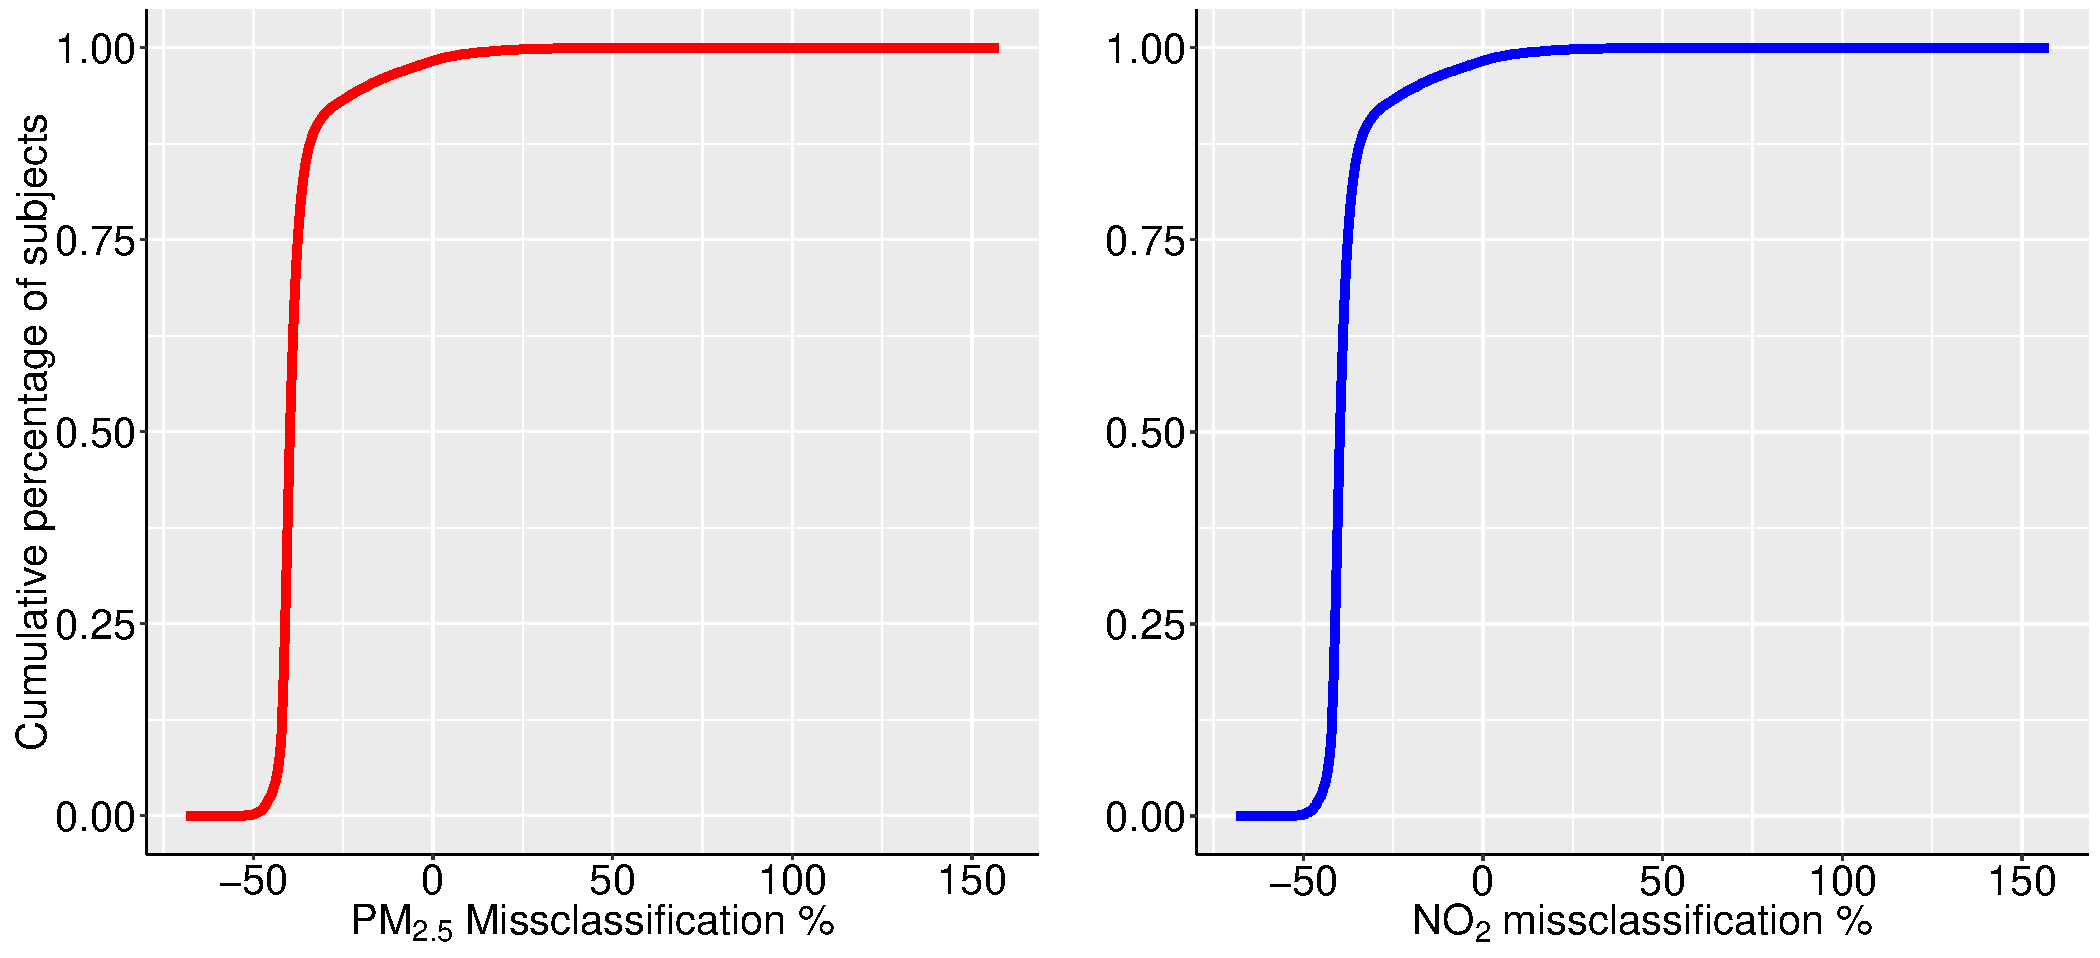
\includegraphics[scale=0.45]{cumulative_missclass_dist}
\caption{Percentage missclassification between LHEM and residential address exposure methods, plotted as a cumulative distribution plot}
\label{fig:cumulative_missclass_dist}
\end{figure}

As is evident from these plots, for the majority of subjects in the dataset, for both PM$_{2.5}$ and NO$_{2}$, the LHEM calculates their exposure as being around 30\% - 50\% lower than the residential address method. There are many ways in which this aspect of the LHEM results could be interrogated, but as an example, a map of the addresses of the subjects where the LHEM calculates an \textbf{increase} in exposure compared to residential address was now created to look for obvious spatial patterns (Figure \ref{fig:address_lhem_increases}).

\begin{figure}[H]
\centering
\includegraphics[scale=0.45]{address_lhem_increases}
\caption{The residential address of subjects whose exposure increased by using the LHEM method compared to residential address}
\label{fig:address_lhem_increases}
\end{figure}

Looking at the NO$_{2}$ map first (shown right), there appears to be fewer people with an increased NO$_{2}$ LHEM exposure in the South-East of London. Whether this is a interesting result and perhaps to do with travel behaviour, or whether it is a result of the number of LTDS subjects being less in that region, is examined by plotting out all the respondants below in Figure \ref{fig:addresses}.

\begin{figure}[H]
\centering
\includegraphics[scale=0.45]{addresses}
\caption{The residential address of subjects whose exposure increased by using the LHEM method compared to residential address}
\label{fig:addresses}
\end{figure}

As can be seen, there appears to be slightly less people in the dataset in the South-East of London, which may explain this pattern (and is reflective of the general population of london (\url{http://londondatastore-upload.s3.amazonaws.com/instant-atlas/borough-profiles/atlas.html})). There could also be additional factors as work, however this would require much more detailed analysis of this aspect of the LHEM, and some sort of regression analysis, so is not attempted in this introduction to the model.

For the PM$_{2.5}$ map, it appears that the people living in Central London are less likely to have increased PM$_{2.5}$ using the LHEM exposure method compared to the residential method, than those living further outside of central London. It seems likely that as high levels of PM$_{2.5}$ are found on the London Underground, and that people living in central London would not need to use the London Underground as frequently or for as long time periods compared to those living in outer London, that this is the reason for this geographical pattern. Although as with the NO$_{2}$ discussion above, this is not investigated further here and is merely suggested as an area for future exploration and as a demonstration of the LHEMs capabilities.

%%%%%%%%%%%%%%%%%%%%%%
\subsection{Pollutant correlation}
\label{subsec:pollutant_correlation}
%%%%%%%%%%%%%%%%%%%%%%

A further area that the LHEM may be of use in health studies is in the separation of health effects from different pollutants. \cite{Brunekreef2007} for example notes that many cohort studies have looked at the negative health effects of NO$_{2}$, but he questions whether NO$_{2}$ is a surrogate for other pollutants such as PM$_{2.5}$, which may be actually causing the health effects. The studies he reviewed found it difficult to look at the relative effects of each pollutant, as they are so strongly correlated. Indeed, using the residential address method, our exposure estimates of the LTDS subjects find that, as the other studies do, NO$_{2}$ and PM$_{2.5}$ are well correlated with a Pearson's R of 0.90 (95\% CI 0.90 to 0.90) (shown left in Figure \ref{fig:correlation_comparisons_no2_pm25} below). In contrast, using the LHEM (Figure \ref{fig:correlation_comparisons_no2_pm25}, right) shows a much more complicated picture of the relationship/correlation between NO$_{2}$ and PM$_{2.5}$, and produces a Pearson's R of 0.66 (95\% CI 0.66 to 0.67). Though as the relationship is not of a linear fashion using the LHEM, Pearson's R is not a valid comparison any longer, and a more complex statistical examination would be required - probably along the lines of a regression model as briefly discussed in Section \ref{subsec:geographical_missclassification} - but again that is not attempted here.

\begin{figure}[H]
\centering
\includegraphics[scale=0.45]{correlation_comparisons_no2_pm25}
\caption{Daily mean exposure to PM$_{2.5}$ v. NO$_{2}$ using residential address exposure method (left) and the LHEM (right)}
\label{fig:correlation_comparisons_no2_pm25}
\end{figure}

This difference between using the LHEM and residential address estimates is an important finding since it has the potential to separate the health effects of NO2 and PM2.5, as part of any ongoing public health research.

%%%%%%%%%%%%%%%%%%%%%%
\subsection{Susceptible groups and exposure}
\label{subsec:susceptible_groups}
%%%%%%%%%%%%%%%%%%%%%%

Studies have shown that the elderly and children are more susceptible to adverse health effects as a result of poor air quality than other age groups (\cite{Wang2015}, \cite{WorldHealthOrganization2013a}). Given this increased risk, the two tables below show summary statistics of exposure to air quality using the LHEM (Table \ref{tab:lhem_comparing_age_categories}) by age-category, for PM$_{2.5}$ and NO$_{2}$, compared to using the residential address method (Table \ref{tab:address_comparing_age_categories}).

\begin{table}[H]
\centering
\begin{tabular}{|l|l|l|l|l|l|}
\hline
                       & \bfseries{Age category}  & \bfseries{Mean}  & \bfseries{Median} & \bfseries{I/Q Range} & \bfseries{5\textsuperscript{th} to 95\textsuperscript{th}} \\ \hline
\multirow{4}{*}{PM2.5} & Child (5-17)             & 13.53 & 13.63 & 13.02 to 14.14    & 12.03-14.62 \\ \cline{2-5} 
                       & Young Adult (18-29)      & 13.63 & 13.74 & 13.10 to 14.24    & 12.14-14.77 \\ \cline{2-5} 
                       & Adult (30-59)            & 13.54 & 13.63 & 12.99 to 14.16    & 12.06-14.66 \\ \cline{2-5} 
                       & Elderly (\textgreater60) & 13.44 & 13.53 & 12.90 to 14.06    & 11.99-14.59 \\ \hline
\multirow{4}{*}{NO2}   & Child (5-17)             & 34.21 & 34.44 & 30.73 to 37.96    & 24.69-42.14 \\ \cline{2-5} 
                       & Young Adult (18-29)      & 35.26 & 35.49 & 31.35 to 39.17    & 25.55-43.59 \\ \cline{2-5} 
                       & Adult (30-59)            & 34.40 & 34.53 & 30.67 to 38.35    & 24.72-42.52 \\ \cline{2-5} 
                       & Elderly (\textgreater60) & 33.53 & 33.58 & 29.76 to 37.52    & 24.13-42.01 \\ \hline
\end{tabular}
\caption{PM$_{2.5}$ and NO$_{2}$ residential address exposure results by age category (n=45,079, concentrations in $\mu \text{g m}^{-3}$)}
\label{tab:address_comparing_age_categories}
\end{table}

\begin{table}[H]
\centering
\begin{tabular}{|l|l|l|l|l|l|}
\hline
                       & \bfseries{Age category}  & \bfseries{Mean}  & \bfseries{Median} & \bfseries{I/Q Range} & \bfseries{5\textsuperscript{th} to 95\textsuperscript{th}} \\ \hline
\multirow{4}{*}{PM2.5} & Child (5-17)             & 8.11    & 8.11   & 7.75 to 8.42    & 7.09-8.96 \\ \cline{2-5} 
                       & Young Adult (18-29)      & 8.92    & 8.39   & 7.91 to 9.03    & 7.2-13.12 \\ \cline{2-5} 
                       & Adult (30-59)            & 8.66    & 8.33   & 7.86 to 8.82    & 7.16-12.32 \\ \cline{2-5} 
                       & Elderly (\textgreater60) & 8.20    & 8.110  & 7.72 to 8.46    & 7.1-9.26 \\ \hline
\multirow{4}{*}{NO2}   & Child (5-17)             & 11.82   & 11.68  & 10.39 to 12.97  & 8.47-15.84 \\ \cline{2-5} 
                       & Young Adult (18-29)      & 13.74   & 13.21  & 11.31 to 15.71  & 9.06-19.66 \\ \cline{2-5} 
                       & Adult (30-59)            & 13.53   & 12.99  & 11.10 to 15.43  & 8.83-19.64 \\ \cline{2-5} 
                       & Elderly (\textgreater60) & 12.17   & 11.77  & 10.36 to 13.43  & 8.34-17.25 \\ \hline
\end{tabular}
\caption{PM$_{2.5}$ and NO$_{2}$ LHEM exposure results by age category (n=45,079, concentrations in $\mu \text{g m}^{-3}$)}
\label{tab:lhem_comparing_age_categories}
\end{table}

This next table (Table \ref{tab:percent_change_comparing_age_categories}) now shows percentage change between the two exposure methods i.e. percentage change between Tables \ref{tab:lhem_comparing_age_categories} and \ref{tab:address_comparing_age_categories}.

\begin{table}[H]
\centering
\begin{tabular}{|l|l|l|l|l|l|}
\hline
                       & \bfseries{Age category}  & \bfseries{Mean}  & \bfseries{Median} & \bfseries{I/Q Range} & \bfseries{5\textsuperscript{th} to 95\textsuperscript{th}} \\ \hline
\multirow{4}{*}{PM2.5} & Child (5-17)             & -40.06\% & -40.50\% & -40.48\% to -40.45\%    & 41.06\%-38.71\% \\ \cline{2-5} 
                       & Young Adult (18-29)      & -34.56\% & -38.94\% & -39.62\% to -36.68\%    & 40.69\%-11.17\% \\ \cline{2-5} 
                       & Adult (30-59)            & -36.04\% & -38.88\% & -39.49\% to -37.71\%    & 40.63\%-15.96\% \\ \cline{2-5} 
                       & Elderly (\textgreater60) & -38.99\% & -40.06\% & -40.16\% to -39.83\%    & 40.78\%-36.53\% \\ \hline
\multirow{4}{*}{NO2}   & Child (5-17)             & -65.45\% & -66.09\% & -66.19\% to -65.84\%    & 65.69\%-62.41\% \\ \cline{2-5} 
                       & Young Adult (18-29)      & -61.03\% & -62.78\% & -63.92\% to -59.89\%    & 64.54\%-54.90\% \\ \cline{2-5} 
                       & Adult (30-59)            & -60.67\% & -62.38\% & -63.81\% to -59.77\%    & 64.28\%-53.81\% \\ \cline{2-5} 
                       & Elderly (\textgreater60) & -63.70\% & -64.95\% & -65.19\% to -64.21\%    & 65.44\%-58.94\% \\ \hline
\end{tabular}
\caption{PM$_{2.5}$ and NO$_{2}$ residential address exposure results by age category (n=45,079, concentrations in $\mu \text{g m}^{-3}$)}
\label{tab:percent_change_comparing_age_categories}
\end{table}

Firstly, these results show that there is more variation in exposure between age groups when using the LHEM compared to using the residential address method. Secondly, they allow us to consider the different exposure of each age group from each method, and lastly they find different patterns e.g. when using the LHEM exposure method, children have the lowest exposure of all age groups to both PM$_{2.5}$ and NO$_{2}$ (and young adults the highest) -- however when using the residential address method, the lowest exposure is found in the elderly instead of the children.

%%%%%%%%%%%%%%%%%%%%%%
%%\subsection{Deprivation and exposure}
%%\label{subsec:deprivation_groups}
%%%%%%%%%%%%%%%%%%%%%%

%%%%\cite{GreaterLondonAuthorityGLA2015}
%%Analysis undertaken for the GLA shows populations living in the most deprived areas are
%%on average currently more exposed to poor air quality than those in less deprived areas.
%%51\% of the Local Super Output Areas (i.e. roughly wards) within the most deprived 1\%
%%of London have concentrations above the NO2 EU limit value. This is in contrast to 1\%
%%above the NO2 EU limit value in the 10\% least deprived areas.

%%\cite{Tonne2008}
%%More deprived areas had higher air pollution concentrations; these areas also experienced greater air pollution %%reductions and mortality benefits compared to the least deprived areas.

%%\cite{Naess2007}
%%Findings from this study suggest that socially deprived neighborhoods have higher exposure to air pollution.

%%\cite{Fernandez-somoano2014}
%%Education and social class were not clearly associated with pollution

%%Not sure of the best way to do this. download index multiple deprivation?
%%Then see whether this holds true for the LHEM or not
%%Could also do for residential address to compare

%%Tempted to drop this section to be honest. or leave it for a bit anyway as this work needs doing for a paper with %%Cathryn Tonne later this year.

%%%%%%%%%%%%%%%%%%%%%%
\section{Discussion}
\label{sec:2Discussion}
%%%%%%%%%%%%%%%%%%%%%%

The LHEM exposure model developed in this chapter, using inputs from the LTDS-X in the previous Chapter, calculates detailed spatial and temporally defined exposure estimates on a level not seen in similar studies. The detail in the inputs separates it in particular, such as the number of participants, the time-activity and demographic detail for them, hourly and spatially resolved CMAQ-Urban data, mass-balance modelling of some of the transport modes, and a very detailed model of indoor exposure. The closest study at this time is that of \cite{Dhondt2012}, who modelled 8000 people, at 15 minute intervals, with only four microenvironments, and less detailed spatial air pollutant inputs. The results in Dhondt were quite different to the results presented here however. For NO$_{2}$ they found that the static address-method was underestimating by an average of 1.2\%, unlike the LHEM which finds an overestimation (13 $\mu \text{g m}^{-3}$ for residential address, and 8.48 $\mu \text{g m}^{-3}$ with the LHEM, meaning the address method is overestimating). Interestingly \cite{DeNazelle2013}, discussed in Section \ref{sec:dynamic_hybrid_models} and in Figure \ref{fig:time_no2_activity_spaces}, found fairly similar NO$_{2}$ results to the LHEM in Barcelona in their measurements-based study. They found that people spend 94\% of their time indoors, and 6\% in transport, where they accumulated 83\% and 7\% of their exposure. Their study population all worked at the University, and as such are likely to fall in the 18-59 age-group categories, and therefore the LHEM results fit very well with these modelled results.

As was demonstrated in the results section \ref{sec:2results}, the LHEM exposure model can allow detailed investigation and calculation of exposure and exposure missclassification. It was used to take a 'first glance' at the relative importance of microenvironments on exposure, the calculation of exposure for different age groups, exposure missclassification, highly exposed people, exposure peaks, whether there were any geographical patterns to exposure missclassification, correlating pollutants, and susceptible groups. Each of these areas was only briefly explored to demonstrate the potential of the model, and further analysis is needed. The model has other uses however, for example each of the LTDS subjects has many more demographic attributes that have not been explored such as ethnicity, income, gender, how many cars the household owns, distance from tube stations etc. that all may play an important role in better understanding exposure. The model can also be used for policy applications which are not explored here, for example what effect would changing 5\% of the subjects journeys from car to walking have on their overall exposure, and how would this vary by age group?

There are a number of ways in which the LHEM could be improved and some elements of the model that might be considered for change in the next iteration.
Firstly, the number of people could be increased, as extra LTDS data is now available from TfL. Adding large numbers of people is likely to increase the strength of the conclusions arrived at, however as many of the exposure results are only marginally different including new subjects may actually change this. It is difficult to say at this stage.
Another area that could be reconsidered is the use of the building I/O ratios from \cite{Taylor2014}. This was an excellent dataset for this research, and to my knowledge unparallelled at this time, however it calculates average ratios on a postcode level, for residential buildings, and therefore may not be suitable for modelling other types of buildings such as office blocks. A new iteration of this dataset might be an option, or indeed developing of an entirely new method.
With regard to the transport modelling, the use of static numbers for the London Underground also seem far from ideal. The figures used for PM$_{2.5}$ were taken from a small number of measurements on one stretch of the Underground by researchers at KCL, when clearly the concentrations will vary on different lines, in different sections of those lines, and perhaps by time of day and season. For NO$_{2}$ the concentrations were taken from a study in Paris, and face similar problems about their applicability to London, and across the network. Refining this aspect of the model will be the focus of the next Chapter.

Perhaps most importantly for the long-term future of this type of model, and perceptions of the results that it produces, is how to validate the estimates. The most likely route to do this would seem to be using personal mobile monitoring, and then comparing this dataset to what the LHEM outputs for similar journeys and days of the subjects.

%Start to talk about how this impacts on London as a whole

%The results presented thus far have been examples of how the LHEM might be useful to an epidemiologist or exposure scientist investigating health effects and air quality. This section now looks at the question of route choice, and how questions that members of the general public might be interested in, and the ways in which the model can answer them. Specifically, route choice and it's effects on exposure is considered and then

%%%%%%%%%%%%%%%%%%%%%%
\section{Conclusions}
\label{sec:2conclusions}
%%%%%%%%%%%%%%%%%%%%%%

%%%\textbf{Time activity}

Results Section \ref{subsec:time_exposure_microenvironments} showed that the LTDS subjects spend most of their time indoors, and thus understanding indoor exposure and being able to model exposure to indoor pollutants (aswell as ingress from outdoor pollutants) is important in understanding exposure in general. With the caveat that the CMAQ-Urban input to the LHEM only models exposure to outdoor pollution, it finds that people are exposed to around 85\% of their daily NO$_{2}$ and 90\% of their daily PM$_{2.5}$ exposure while indoors - although this varied slightly by age group, with children and the elderly accumulating more of their daily exposure from the indoors environment that adults and young adults, due to the slightly increased time that they spend indoors, and naturally a reflection of this, the increased time that adults and young adults spend in transport in environments of higher concentrations that indoors. Comparing exposure in transport modes is difficult, as except for the underground, they are a function of the outdoor concentrations. However on a time/exposure basis, active travel can be seen to result in lower exposure than passive travel.

%%%\textbf{Exposure comparisons}

The different exposure values found in results Section \ref{subsec:comparing_exposure_methods} should help epidemiologists understand that the means and ranges of exposures that are currently being used in health studies are perhaps not appropriate, and that they may be over-estimating exposure across the population (and using incorrect ranges). The LHEM finds that estimates based on monitoring sites, postcodes or residential address are all overestimating exposure for both PM$_{2.5}$ and NO$_{2}$, by varying degrees depending on the method in comparison. Interestingly, when comparing postcode and residential address estimates across the 45,079 people, they are found to be almost identical. Given this, perhaps the recent drive for individual residential addresses for completing exposure analysis is unrequired, and postcode estimates are sufficient to reflect the variation in exposure using static analysis methods (although studies discussed in the Introduction typically took annual averages, rather than the hourly variation that CMAQ-Urban models). When the LHEM exposure estimates are plotted against residential address estimates, with the points coloured by whether people left their house during the day, this factor appears to be the main reason for the differences between the LHEM and residential address method exposure estimates (instead of perhaps the indoor-outdoor ratios, which would only result in lower estimates but with the same overall profile). Introducing the LHEM to exposure estimates creates peaks and ranges in a persons daily exposure that are not seen using other methods.

%%%\textbf{Highly exposed people}

In results section \ref{subsec:highly_exposed_people}, it was demonstrated how the LHEM can investigate the numbers of people who are accumulating daily mean exposures above the WHO limits for PM$_{2.5}$ and NO$_{2}$. As the static models of exposure do not take account of the subjects movements, or normally the effects of exposure being different when people are indoors, if a subjects house happens to be in an area of very high concentrations then that persons mean exposure is taken to be high. When actually the LHEM (compared to residential exposure method) demonstrates that when the subjects daily activities are taken into account, their daily mean exposure is actually (generally) lower. The result of this with the LHEM, is that much fewer subjects are found to be living in areas above the WHO limits.

%%%\textbf{Exposure peaks}

As the LHEM calculates exposure on a minute-by-minute basis, Section \ref{subsec:exposure_peaks_by_age_group} showed how it can also be used to consider much shorter periods of high exposure in a subjects day that other models are generally unable to do. Using this aspect of the LHEM, we find that the LTDS subjects are exposed to levels of 'unacceptable' (as defined by the WHO) PM$_{2.5}$ and NO$_{2}$ levels for between 13.1\% and 16\% and 1.3\% and 3.8\% respectively, depending on age group.

%%%\textbf{Geographical missclassification}

By calculating the percentage difference between the residential address method, and the LHEM method, we were able to see how for most people the difference in exposure is between (approximately) -50\% and -20\%, but how there were was a long-tail of distributions and some people were found to have higher mean exposure estimates when using the LHEM. The people with higher LHEM than residential exposure estimates were mapped, to see if there was any specific geographical distribution to these results, but none was apparent.

%%%\textbf{Pollutant correlation}

The LHEM was now used to see whether PM$_{2.5}$ and NO$_{2}$ exposures were found to be correlated, as they are in many other health effect studies (discussed in Section \ref{subsec:pollutant_correlation}. First the residential PM$_{2.5}$ and NO$_{2}$ were checked for correlation to see if the data and subjects in this research were similar to others, and they were found to have a R\textsuperscript{2} of 0.90, confirming that they were. The same analysis using the LHEM however resulted in an lower correlation of 0.66 i.e. poorly correlated. However there actually appear to be two different correlations within the scatter-plot, and thus this requires further investigation. This difference between pollutants using the LHEM may allow future health studies to better be able to estimate the differences in health effects from individual pollutants.

%%%\textbf{Susceptible groups}

Finally the LHEM was used to investigate how exposure varies by age groups in Section \ref{subsec:susceptible_groups}. It demonstrated how each age group has fairly similar ranges and means of exposure, and similar missclassification between the LHEM and residential exposure estimates.